\chapter{Xây dựng UIT-OWL Editor}
\paragraph{Giới thiệu} Qua các chương trước, chúng em đã trình bày các cơ sở lý thuyết từ Semantic Web, Ontology Web Language và giới thiệu khái quát về OWL-API, Vaadin Framework- 2 công cụ chính xây dựng nên ứng dụng chỉnh sửa và phát triển Ontology trên Web mà chúng em tạm gọi là UIT-OWL Editor. Trong chương này, chúng em sẽ trình bày một cách chi tiết nhất có thể về quá trình xây dựng và phát triển nên ứng dụng này.
\section{Bố cục của ứng dụng}
\begin{figure}[h!]
	\centering
	\frame{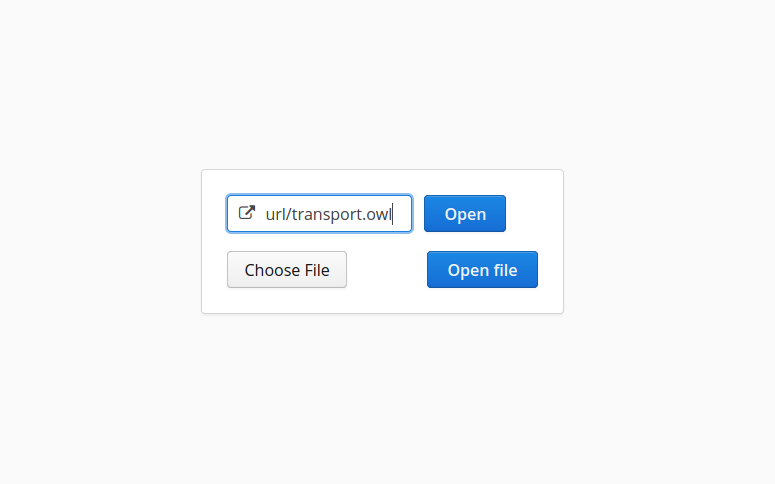
\includegraphics[width=100mm]{Figures/owleditor_entryview.png}}
	\caption{EntryView của UIT-OWL Editor\label{overflow}}
\end{figure}
\begin{figure}[h!]
	\centering
	\frame{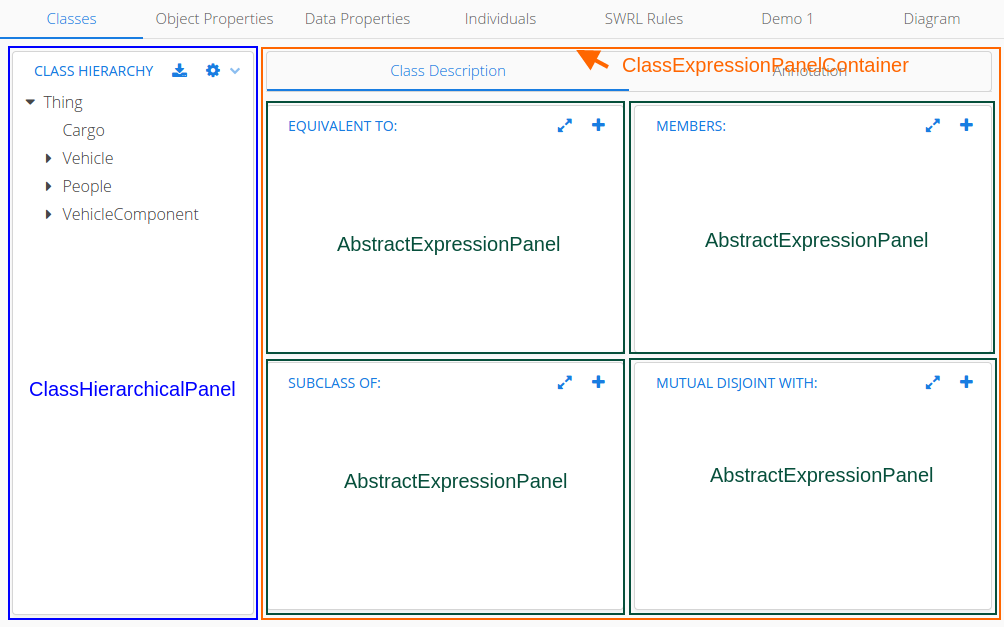
\includegraphics[width=150mm]{Figures/owleditor_mainview.png}}
	\caption{MainView của UIT-OWL Editor\label{overflow}}
\end{figure}
%
\subsection{Các view chính}
Ứng dụng UIT-OWLEditor chỉ gồm 2 View chính:
\begin{description}
\item[Entry View] tương đương với lớp \textit{vn.edu.uit.owleditor.EntryView} trong mã nguồn, là nơi chúng tập nhập vào URL của file OWL2 Ontology hoặc tải file OWL2 Ontology với các định dạng được trình bày trong chương 2.
\item[Main View] tương đướng với lớp \textit{vn.edu.uit.owleditor.MainView} trong mã nguồn,là giao diện chính của ứng dụng UIT-OWL Editor.
\end{description}
%
\subsection{Các tabsheet trong Main View}
Trong \textbf{MainView} sử dụng Component TabSheet các chứa các Tab tương ứng với các thực thể trong OWL2 Ontology, duy chỉ có 2 Tab cuối dùng để dùng làm demo tính năng phân loại là Tab Demo và Tab cuối cùng là Diagram dùng để vẽ các diagram, đồ thị về phân cấp các đối tượng trong OWL 2 Ontology.

% Class Tab
\subsubsection{Tab Classes} 
\begin{figure}[h!]
	\centering
	\frame{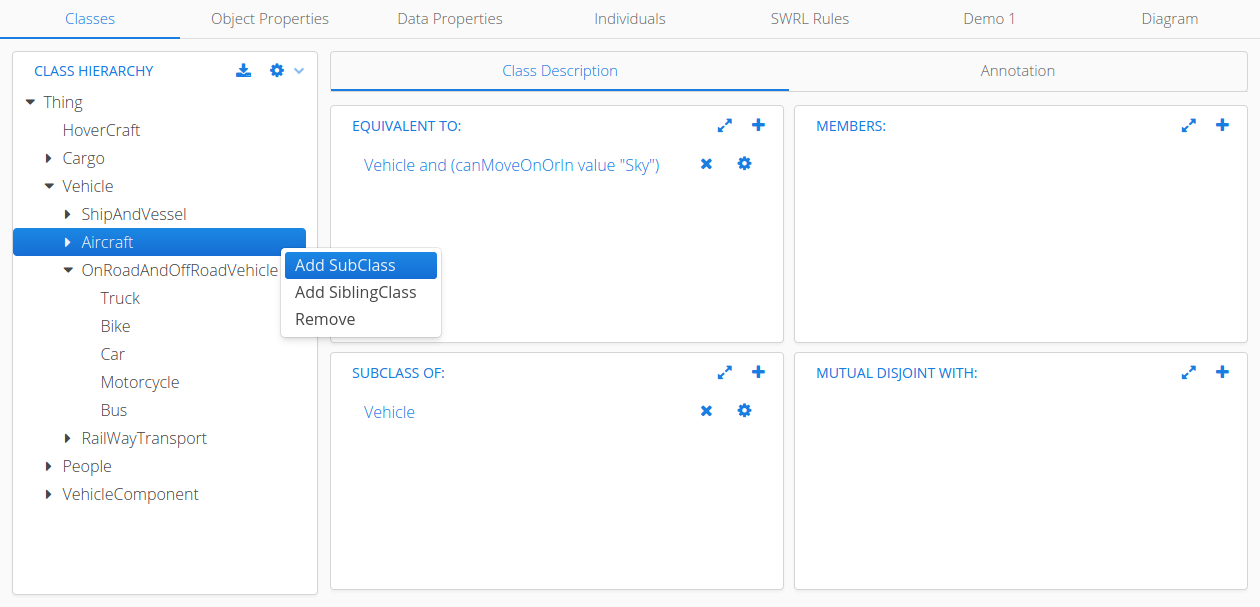
\includegraphics[width=150mm]{Figures/owleditor_classSheet.png}}
	\caption{Class Tab trong UIT-OWL Editor\label{overflow}}
\end{figure}
Tương ứng với lớp \verb|vn.edu.uit.owleditor.view.ClassesSheet| trong mã nguồn. Giao diện sử dụng HorizontalLayout của Vaadin gồm 
\begin{enumerate}
\item Panel bên phải là ClassHierachicalPanel có một cấu trúc dạng cây với các node chính là các lớp nằm trong OWL2 Ontology, với các chức năng thêm node và xóa node.
\item Các panel nhỏ bên phải được chứa trong lớp ClassExpressionPanelContainer, mỗ panel thể hiện một mô tả tương ứng với tên của panel đó.
\end{enumerate}	

% Object Property Tab
\subsubsection{Tab Object Properties}  
\begin{figure}[h!]
	\centering
	\frame{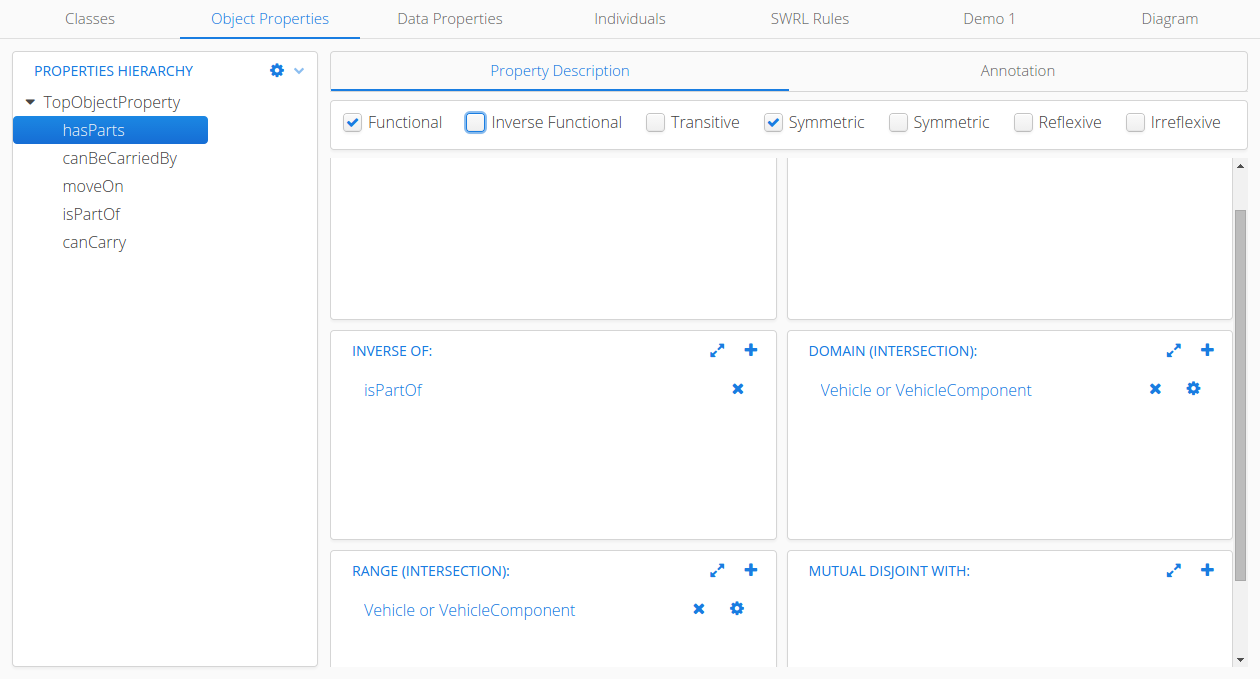
\includegraphics[width=150mm]{Figures/owleditor_opSheet.png}}
	\caption{Object Properties Tab trong UIT-OWL Editor\label{overflow}}
\end{figure}
Tương ứng với lớp \verb|vn.edu.uit.owleditor.view.ObjectPropertiesSheet| trong mã nguồn. Giao diện sử dụng HorizontalLayout của Vaadin gồm 
\begin{enumerate}
\item Panel bên phải là ObjectPropertyHierachicalPanel có một cấu trúc dạng cây với các node đại diện cho các thuộc tính đối tượng trong OWL2 Ontology, với các chức năng thêm node và xóa node tương tự như của Tab Classes.
\item Một dãy các \textit{CheckBox} dùng để thêm/xóa với các phát biểu trong mục 3.3.6.2 liên quan đến thuộc tính đối tượng được chọn bên trong cấu trúc cây ở bên phải.
\item Các panel nhỏ bên phải được chứa trong lớp ObjectPropertyExpressionPanelContainer, mỗ panel thể hiện một mô tả tương ứng với tên của panel đó về thuộc tính đối tượng đang được chọn trên cấu trúc cây.
\end{enumerate}	





\section{Cấu trúc package của ứng dụng}
\subsection{vn.edu.uit.owleditor}
Chứa các đối tượng có vai trò là nơi đầu tiên code được thực thi khi người dùng gõ vào URL của ứng dụng. Gồm các đối tượng quan trọng sau
\begin{description}
\item[OWLEditorUI] là đối tượng được mở rộng (thừa kế) lớp \verb|UI| của Vaadin với chứng năng là nạp các component từ Entry 
\end{description}